\chapter{Sicurezza}\label{sicurezza}

\section{Reti P2P in genere}\label{reti-p2p-in-genere}

Una rete di computer, di qualsiasi tipo essa sia, richiede    necessariamente un certo livello di sicurezza. Questo è ancora più vero per reti pubbliche in cui chiunque può inserirsi, come le reti P2P che
si appoggiano a Internet.
Tali reti sono un bersaglio particolarmente ghiotto per gli attaccanti proprio a causa della loro maggiore forza: il grande numero di utenti,
che equivale ad un grande numero di possibili bersagli. Ogni rete P2P deve quindi confrontarsi con la certezza che alcuni dei suoi nodi siano
malevoli.  Data la grande varietà di reti P2P, è necessario specificare cosa intendiamo per ``reti P2P in genere''. Il modello \cite{vulnerabilities} a cui si farà riferimento consiste nelle seguenti componenti di base:

\begin{itemize}
\itemsep1pt\parskip0pt\parsep0pt
\item
  Uno spazio degli ID composto da b bits.
\item
  Un sistema di mappatura degli ID.
\item
  Un sistema di routing, che utilizza una chiave per inoltrare un   messaggio alla sua destinazione. Questo include una serie di regole   per il churn.
\end{itemize}

%TODO vedere se usare la documentazione del prof per descrivere i modelli di rete P2P

Basandoci sul modello di rete OSI, classifichiamo gli attacchi come di basso, medio e alto livello, a seconda della vicinanza al livello di comunicazione fisico: più il livello dell'attacco è alto, più si basa sul software invece che sull'hardware.

Visto che le reti P2P sono costruite sulla base di altre reti, i livelli ISO/OSI a cui siamo interessati sono il livello applicativo (per il P2P vero e proprio) e il livello di comunicazione (per attacchi basati su TCP e IP).

\begin{figure}[htbp]
\centering
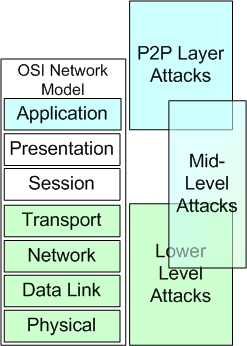
\includegraphics[scale=0.5]{vulnerabilities_p2p-001.PNG}
\caption{Livelli di attacco in confronto con lo stack ISO/OSI.\label{vulnerabilities_p2p-001}}
\end{figure}

\subsection{Attacchi di Basso Livello}\label{attacchi-di-basso-livello}

\subsubsection{Denial of Service (DoS)}\label{denial-of-service-dos}

Uno degli attacchi più basilari che interessa praticamente ogni tipo di rete. Consiste nel bloccare i servizi offerti da uno specifico bersaglio. Si tratta di un attacco estremamente comune esistente in infinite varianti, ma nel caso di P2P la sua versione più semplice consiste nel flood. Consiste nell'estremizzare quanto descritto nel query flood\footnote{Confrontare sezione \ref{query-flooding}}: inondare la rete di pacchetti, legittimi o creati ad-hoc, in modo da ostacolare la normale comunicazione tra i nodi. Semplice, ma estremamente efficace.

Una variante ancora più efficace, e resa tale proprio dalla natura distribuita delle reti P2P, consiste nel \textbf{Distribute Denial of Service} (DDoS). Come dice il nome, la differenza sta nel fatto che l'attaccante non è un singolo nodo bensì un insieme di nodi. Il vantaggio in questa tecnica, oltre che nell'immenso numero di pacchetti che inondano la rete, sta nell'anonimato che circonda l'attaccante. Spesso infatti i nodi che a tutti gli effetti inviano i pacchetti sono inconsapevoli di essere parte dell'attacco e manipolati remotamente da un attaccante. Questo aggiunge un ulteriore strato tra l'attaccante e i nodi legittimi che tentano di impedire l'attacco.

Gli attacchi DoS e DDoS diventano tanto più probabili quanto più è vasta la rete, non solo per il maggior numero di nodi compromettibili per un DDoS, ma anche per le politiche aziendali attuate da molte società e provider. Infatti, più la rete è diffusa, più è probabile che firewall aziendali ne limitino l'accesso ai propri utenti e che ISP nazionali ne limitino l'utilizzo. Questo costringe gli utenti a piazzarsi al di fuori di tali reti protette per poter usufruire della rete P2P, e quindi ad esporsi maggiormente agli attacchi.

\paragraph{Contromisure al DDoS}\label{contromisure-al-ddos}

Il primo problema consiste nell'identificare i DDoS. I sintomi di un DDoS sono del tutto identici a quelli di un normale elevato traffico di rete, in particolare quando i pacchetti usati sono legittimi e non forgiati ad-hoc per l'attacco. Inoltre in un DDoS non tutti i nodi sono stati creati appositamente per attaccare, spesso sono nodi legittimi che vengono utilizzati dall'attaccante per far rimbalzare i suoi pacchetti di attacco. Questi due fattori combinati rendono di fatto \emph{impossibile} bloccare tutti gli attacchi DoS.

Esiste però una tecnica ampiamente diffusa per rendere poco pratico il DoS, o almeno per rallentarlo in maniera drastica. Si tratta del \textbf{pricing}, una tecnica che limita la velocità alla quale i nodi possono fare richieste alla rete. Se un nodo deve fare richieste ad un altro nodo (ad esempio, una query per un file), il nodo risponde con richieste di calcoli di hash, esattamente gli stessi calcoli necessari per creare un blocco in Bitcoin. Solo dopo aver risolto il calcolo ed inviata la risposta, la richiesta viene presa in considerazione, tutte le altre comunicazioni inviate nel frattempo vengono scartate, scoraggiando quindi qualsiasi richiesta invadente.

\subsubsection{Attacco Man-in-the-Middle (MitM)}\label{attacco-man-in-the-middle-mitm}

Questo attacco consiste nell'inserimento dell'attaccante tra due nodi della rete, in modo che tutte le comunicazioni tra i due nodi passino attraverso l'attaccante. L'attacco è irrilevabile fin tanto che l'attaccante rimane passivo. Una volta ottenute tutte le informazioni che desidera, l'attaccante può diventare attivo modificando i messaggi che vengono scambiati oppure forgiandone di propri spacciandosi per uno o entrambi dei nodi. Inoltre, dato che l'attaccante può influenzare la visione che i due nodi hanno del resto della rete, può creare false identità per simulare messaggi legittimi.

Se questo attacco viene effettuato al livello di rete, l'attaccante è in grado di vedere tutto ciò che passa tra i due nodi e, essendo questo livello inferiore a quello P2P, l'attaccante non ha nessun problema nel creare qualsiasi tipo di pacchetto P2P egli desideri.

Come il DoS ma in misura estremamente maggiore, le reti P2P sono un bersaglio goloso per questo genere di attacchi. Questo perché è difficile inserirsi tra due nodi in una rete normale, ma in una rete P2P è estremamente banale: tali reti infatti non hanno nessun controllo su come sono localizzati i nodi e sono quindi \emph{estremamente} vulnerabili al MitM.
%TODO anche qui la stessa roba del tipo di reti del libro del prof
Dato che l'attaccante può piazzarsi dove vuole all'interno della rete, gli attacchi risultano essere molto specifici e deterministici, fino anche ad impedire ad un determinato nodo di accedere ad un altro nodo.

\subsubsection{Contrastare il Man-in-the-Middle}\label{contrastare-il-man-in-the-middle}

Il metodo principale per difendersi dal MitM è rendere tale attacco il più infruttuoso possibile. In una rete senza nodi privilegiati (ad esempio un server centrale, un supernodo o un'autorità centrale di autenticazione), il MitM si limita a compromettere la sicurezza tra due soli nodi nella rete, senza minacciare per nulla il resto dei nodi \footnote{almeno fino a quando la perdita di tre nodi (due vittime e un   attaccante) risulta tollerabile per la rete, il che è vero per tutte   quelle reti ampiamente diffuse.}.

Molte reti (non bitcoin) sfruttano nodi privilegiati per affrontare altre minacce o come parte integrante della loro struttura, e anche nelle reti maggiormente distribuite è possibile effettuare un attacco MitM su larga scala (vedi \ref{attacco-eclipse} più avanti).

Il metodo più diffuso per evitare la fuoriuscita di informazioni nella comunicazione tra due nodi è la cifratura a chiave pubblica. Con tale sistema si garantisce l'origine del messaggio, il fatto che non è stato alterato in alcun modo e, volendo, fornisce anche un metodo per evitare che una terza parte non autorizzata possa leggerne il contenuto. L'implementazione di questo semplice meccanismo rende praticamente inutile qualsiasi tentativo di MitM tra due nodi.

\subsection{Attacchi di Medio Livello}\label{attacchi-di-medio-livello}

\subsubsection{Worms}\label{worms}

Un worm è un programma auto-replicante simile a un virus che, a differenza di questo, è indipendente da altri programmi presenti sul sistema. La minaccia rappresentata da un worm è decisamente significativa per una rete P2P, in quanto si diffondono a tutti i nodi della rete tramite vulnerabilità presenti ad un livello più basso rispetto a quello della rete stessa. Pur non essendo legati direttamente al P2P, i worm vengono diffusi in modo capillare da esso principalmente a causa di come il P2P viene implementato. In molte architetture infatti i nodi per comunicare tra loro devono avere installato lo stesso software. Ciò significa che quando questo software ha una certa vulnerabilità (ad esempio, un buffer overflow), tutti i nodi della rete sono vulnerabili. Quindi mentre un worm ``normale'' deve effettuare una scansione dell'intera rete per trovare degli host vulnerabili, un worm P2P deve solo guardare le tabelle di routing e infettare tutti i nodi vicini, diffondendosi esponenzialmente: in confronto ai worm normali, i worm P2P infettano l'intera rete in modo praticamente istantaneo.

Oltre alla grande velocità di diffusione, il fatto che molte reti P2P siano concepite per il file-sharing e abbiano quindi una grande abbondanza di banda, consente al worm P2P di avere dimensioni maggiori e di essere quindi capace di azioni ed attacchi molto più complicati rispetto ad un worm normale, a volte grande solo come un pacchetto TCP/IP. Molti nodi sono inoltre spesso computer personali di utenti normali che utilizzano quotidianamente Internet. Worm sufficientemente complessi sono in grado di monitorare l'attività dell'utente anche al di fuori della rete P2P e di accedere a dati quali numero di carta di credito, password di account, ecc., rendendo le reti P2P un bersaglio di estremo valore.

Infine, i worm possono usare la rete come uno strumento. Si è parlato prima parlando del DDoS (nella sezione \ref{denial-of-service-dos}) di come un nodo qualsiasi possa diventare un ignaro vettore di attacco. I worm sono il modo in cui questo viene reso possibile: il worm contiene tutto il codice necessario ad effettuare l'attacco, oltre al codice per replicare se stesso negli altri nodi.

\paragraph{Contrastare i Worm}\label{contrastare-i-worm}

Il modo principale è mantenere le applicazioni sicure: senza una vulnerabilità comune un worm non può diffondersi in modo efficace. La sicurezza di un software dipende dal modo in cui esso è stato programmato, ad esempio per ridurre il rischio di buffer overflow è possibile usare linguaggi fortemente tipati.

Per ridurre invece l'efficacia di un worm si può decentralizzare il più possibile la rete evitando di implementare nodi privilegiati e/o utilizzare sistemi operativi \textbf{hardened}. OpenBSD dalla versione 3.8 per esempio utilizza indirizzi pseudocausali in fase di allocazione della memoria, rendendo quindi difficile sfruttare vulnerabilità presenti nei vari applicativi.

Ma il modo più pratico per difendersi dai worm è mantenere aperta la rete. Ciò significa basarsi su standard diffusi ed aperti per i propri applicativi. Rilasciare i protocolli al pubblico e distribuire il codice dei propri software incoraggia altri sviluppatori ad una analisi critica, il che porta alla più tempestiva scoperta di vulnerabilità ed alla rapida creazione di patch, bug-fix e fork più robusti del software in questione. Inoltre, con opportune licenze, ogni sviluppatore può creare il proprio client per interfacciarsi con la rete costringendo un attaccante a creare un worm specifico per ogni versione di ogni client, e a mantenere tale worm aggiornato mano a mano che nuove vulnerabilità vengono scoperte e risolte o nuovi client implementati. Con una grande varietà di client a disposizione, non tutti i nodi saranno vulnerabili allo stesso identico difetto presente in un altro client.

\subsection{Attacchi al livello P2P}\label{attacchi-al-livello-p2p}

\subsubsection{Comportamento scorretto}\label{comportamento-scorretto}
 Non si tratta di danneggiare una rete intera o un singolo nodo, bensì di trarre il massimo profitto offrendo minima collaborazione. Questo comportamento viene definito genericamente \textbf{attacco razionale}. La terminologia si basa sull'assunzione che dietro ogni nodo ci sia un utente razionale che per istinto tenta di trarre il massimo beneficio con il minimo sforzo. Ad esempio nell'ambito della rete BitTorrent un utente scarica un file eliminandolo dalla condivisione non appena completo, oppure riduce ai minimi termini la banda in upload massimizzando quella in download: tale comportamente viene definito significativamente \textbf{leeching}, letteralmente \emph{sanguisuga}.

Ci sono molte ragioni per cui un nodo debba comportarsi in questo modo:

\begin{itemize}
\itemsep1pt\parskip0pt\parsep0pt
\item
  Per preservare la banda in upload, spesso molto limitata dagli ISP.
\item
  Per motivi legali, in special modo dove la condivisione di contenuti   protetti dal copyright può risultare in un'azione legale nei confronti   del nodo che condivide. Data la natura aperta delle reti, spesso è   molto facile risalire all'origine di un contenuto.
\item
  Per istinto: molte persone, se viene lasciata loro possibilità di   scelta, tendono a non cooperare per il solo benificio di aiutare la   comunità a cui appartengono, non importa quanto minimo sia il costo   che comporta loro.
\end{itemize}

Come descritto, due sono i metodi in cui ci può implementare questo ``attacco'': riducendo le risorse a disposizione della rete oppure riducendo il contenuto condiviso.

\paragraph{Contrastare i comportamenti scorretti}\label{contrastare-i-comportamenti-scorretti}

Ogni rete deve implementare il suo diverso meccanismo per favorire la collaborazione tra i peer: in Bitcoin ci sono le transaction fee, Napster utilizzava un meccanismo di reputazione che favoriva gli utenti che condividevano di più, Samsara (una rete di backup distribuito) consente ad un utente di utilizzare uno spazio su un altro nodo solo pari a quello che l'utente mette a disposizione per gli altri nodi.

Un esempio encomiabile è quello di BitTorrent: il protocollo è disinteressato al numero di file condivisi da un utente o dal contenuto di per se, ma si interessa solamente di quante risorse vengono condivise. Secondo il protocollo BitTorrent i file da condividere vengono suddivisi in parti (\textbf{chunk}) di lunghezza variabile che vengono barattati tra i nodi: più un nodo è disposto a dare, più si vedrà restituire. In pratica, più è alta la velocità di upload, più gli altri nodi assegneranno banda a quel nodo, aumentandone la velocità di download.

\subsubsection{Attacco Sibilla}\label{attacco-sibilla}

Si ha questo attacco quando una singola entità malevola rappresenta un grande numero (spesso estremamente elevato) di utenti in una rete P2P con l'obiettivo di assumere il controllo di un segmento della rete. L'attacco si implementa con l'attaccante che tenta di creare un grande numero dei nodi a lui vicini. L'attacco diventa più efficace se l'attaccante è in grado di decidere dove posizionarsi nella rete, in quanto potrebbe aver bisogno di meno nodi per poter causare gravi danni alla rete. Con molti nodi a propria disposizione è possibile controllare tutti i messaggi che passano per il segmento formato dai nodi in questione. Questo attacco è inoltre un \textbf{attacco gateway}, il che sta ad indicare una categoria di attacchi solitamente usati come passo preliminare per attacchi su vasta scala di altro tipo, come per esempio l'attacco Eclipse descritto nella sezione \ref{attacco-eclipse}.

\paragraph{Contromisure all'attacco Sibilla}\label{contromisure-allattacco-sibilla}

La natura aperta delle reti P2P gioca a favore di questo tipo di attacco: senza un'autorità centrale è impossibile fermare completamente un attacco Sibilla. Il meglio che si può fare è renderlo impraticabile.

Per rallentare un attacco si può usare lo stesso metodo usato con gli attacchi DoS: il pricing (confrontare la sezione \ref{denial-of-service-dos}).
Il grande numero di calcoli richiesti per unire molti nodi alla rete può richiedere all'attaccante più tempo di quanto sia disposto ad impiegarne. Se inoltre la rete implementa una sorta di tempo massimo durante il quale un nodo mantiene un certo identificativo, tutti gli attacchi hanno un tempo massimo entro il quale devono essere portati a termine, dopo di che i nodi creati dovranno ricollegarsi alla rete e quindi si dovranno ripetere tutte le pratiche del pricing.

\subsubsection{Attacco Eclipse}\label{attacco-eclipse}

L'obiettivo di questo attacco è di separare la rete in due o più partizioni. Quando l'attacco ha successo, tutte le comunicazioni tra le due partizioni devono passare attraverso un singolo nodo malevolo. In pratica questo risulta in un attacco Man-in-the-Middle su vasta scala eseguito a livello applicativo e non a livello di rete, con tutte le potenzialità del MitM normale. Per eseguire l'attacco bisogna piazzare i propri nodi in punti di routing strategici che esistono tra le due partizioni che si vogliono creare. Un attacco Eclipse di successo può distruggere qualsiasi rete P2P, soprattutto quelle che non si curano molto di mantenere tabelle di routing efficienti, perché i nodi finti possono essere posizionati in modo da riempire i vuoti nelle tabelle di routing di ogni altro nodo.

\paragraph{Contromisure ad Eclipse}\label{contromisure-ad-eclipse}

Data la similarità di Eclipse con il MitM, le contromisure sono anche similari: cifratura a chiave pubblica. Tuttavia, sebbene MitM non sia una minaccia per la rete, le dimensioni di Eclipse lo rendono estremamente pericoloso anche in caso di cifratura a chiave pubblica. Se i messaggi illeciti indirizzati ai nodi legittimi vengono bloccati, le due partizioni create da Eclipse rimangono di fatto isolate. Con abbastanza nodi piazzati in punti strategici della rete, è possibile creare quante divisioni si desidera, riducendo quindi le dimensioni della rete.

Come per l'attacco Sibilla, è importante impedire ad un attaccante di decidere dove piazzare i suoi nodi. Questo significa che sarà richiesto un elevato numero di nodi per avere una speranza di ottenere sufficiente controllo per poter creare una partizione. Per cui è importante notare che con un attacco Sibilla sufficiente grande è \emph{sempre} possibile eseguire un attacco Eclipse.

\subsection{Contromisure generali}\label{contromisure-generali}

Si è quindi visto come, oltre alle caratteristiche di tolleranza ai guasti e grande scalabilità che ne rappresentano la base del design, le reti P2P devono anche essere progettate per difendersi dagli attacchi. Solo in questo modo una rete potrà consentire ad ogni nodo di collegarsi e realizzare in pieno il concetto di collaborazione che sta alla base.

In particolare i progettisti di reti P2P dovrebbero implementare le seguenti caratteristiche:

\begin{itemize}
\itemsep1pt\parskip0pt\parsep0pt
\item
  L'impossibilità per un nodo di decidere in che punto della rete   piazzarsi.
\item
  Un limite per la velocità di churn per i nuovi nodi.
\item
  Limitare la velocità di scambio di messaggi tra i nodi, ad esempio   con un princing.
\item
  Utilizzare la crittografia a chiave pubblica per garantire solo   messaggi legittimi tra i nodi.
\item
  Usare ed implementare solo standard aperti, per diversificare il   software a disposizione degli utenti ed irrobustire quelli esistenti.
\end{itemize}

Se queste caratteristiche vengono implementate, allora tutti gli attacchi fin qui descritti perdono gran parte della loro efficacia, ripagando con la sicurezza il costo che richiede la loro realizzazione.

\section{La rete Bitcoin}\label{la-rete-bitcoin}

\subsection{Attacchi basati sulla velocità}\label{double-spending}

Come descritto dallo stesso autore in \cite{bitcoin}, una transazione Bitcoin viene fissata nella blockchain e quindi resa (tecnicamente \ref{attacchi-hashrate}) immutabile solamente quando inclusa in un blocco. Dato che la rete si autoregola per trovare un blocco ogni 10 minuti circa, è evidente come questo sia il tempo minimo di attesa da lasciar trascorrere per avere la certezza che una transazione sia andata a buon fine. Questo meccanismo di verifica è eccellente per commerci in cui la consegna del servizio è dilazionata nel tempo rispetto al pagamento, come ad esempio il caso dell'acquisto online, ma risulta inefficace nel caso in cui la consegna del servizio richiesto sia rapida, nell'ordine dei 30 secondi: mentre l'attesa è un problema personale, la mancata conferma del buon esito della transazione espone il commerciante al rischio di non ricevere il pagamento subendo un attacco doppia-spesa. Con il termine \emph{doppia-spesa} ci si riferisce al caso in cui un utente $\mathcal{A}$ può reclamare la proprietà e spendere presso un diverso indirizzo le stesse BTC precedentemente inviate all'indirizzo di un venditore $\mathcal{V}$ in cambio di servizi che non vengono quindi retribuiti.\\
Karame, Androulaki e Capkun, nella loro ricerca \cite{doublespendig_fast} hanno analizzato il problema da un punto di vista formale evidenziandone le criticità e proponendone alcune soluzioni, in aggiunta ai consigli che gli stessi sviluppatori, ben consapevoli del problema, forniscono ai venditori che intendono usare Bitcoin per pagamenti rapidi.
La prima cosa che i ricercatori fanno notare è che sebbene i tempi di conferma delle transazioni in Bitcoin siano modellabili come una distribuzione geometrica traslata a sinistra(\ref{misurazioni}) in cui i tempi di conferma medi siano intorno ai 10 minuti, la deviazione standard raggiunge i 15 minuti: tali misurazioni sono basate sui primi 153260 blocchi (fino al 14 Novembre 2011) che mostrano inoltre come solo il 64\% di quei blocchi sia stato generato in meno di 10 minuti, mentre per il rimanente 36\% sono stati necessari tra i 10 e 40 minuti. Come si vede, il problema è rilevante per gli scambi commerciali che devono per forza di cose essere molto rapidi.

\subsubsection{Modello di attacco}

Come accennato, si considera il caso in cui un attaccante/acquirente $\mathcal{A}$ desideri ottenere un servizio rapido da un venditore $\mathcal{V}$ senza spendere le proprie BTC, ovvero facendo credere a $\mathcal{V}$ di essere stato pagato salvo poi deviare il pagamento verso un altro indirizzo impedendo a $\mathcal{V}$ di reclamare le BTC che gli spettano.\\
Si immagini quindi che $\mathcal{A}$ crei una transazione $\tau_\mathcal{V}$ diretta a $\mathcal{V}$ ed entro pochissimi secondi crei una seconda transazione $\tau_\mathcal{A}$ che sfrutti lo stesso identico input della precedente ma che come destinatario abbia un indirizzo sotto il controllo di $\mathcal{A}$. Quando $\mathcal{V}$ riceve la prima transazione, cosa che richiede mediamente 3 secondi, nel suo client può verificare come l'indirizzo del mittente e l'ammontare siano corretti e fornire quindi il servizio richiesto. Ma ad essere confermata tramite l'inclusione in un blocco sarà la seconda $\tau_\mathcal{A}$ che impedirà in modo irreversibile a $\mathcal{V}$ di ricevere il suo pagamento. Infatti se le due transazioni vengono inviate molto vicine nel tempo, solamente una di esse verrà inclusa in un blocco in quanto i nodi considerano invalide transazioni che hanno lo stesso input di transazioni precedentemente ricevute.\\
Impostando $\mathcal{X} \in \left[ \mathcal{A}, \mathcal{V} \right]$ e denotando con $t^\mathcal{X}_i$ l'istante in cui il nodo $i$ riceve $\tau_\mathcal{X}$ e con $t^\mathcal{X}_\mathcal{V}$ l'istante in cui $\mathcal{V}$ riceve $\tau_\mathcal{X}$ si hanno due condizioni necessarie da rispettare per un attacco doppia-spesa di successo. Ovviamente questi requisiti sono sufficienti solo nel caso in cui il commerciante verifichi solamente la ricezione della transazione sul proprio client e non sfrutti altre tecniche per verificare od eliminare gli attacchi doppia-spesa. Mentre queste assunzioni rispecchiano le attuali implementazioni dei client, non tengono conto dei consigli dati a coloro che intendono aprire un'attività commerciale Bitcoin basata sui pagamenti rapidi, che verranno descritti più avanti.

\paragraph{1: $t^\mathcal{V}_\mathcal{V} < t^\mathcal{A}_\mathcal{V}$}

Se tale requisito non viene rispettato allora $\mathcal{V}$ riceverebbe prima $\tau_\mathcal{A}$ rifiutando $\tau_\mathcal{V}$ e quindi richiedendo a $\mathcal{A}$ un nuovo pagamento o rifiutandosi di offrire il servizio.\\
$\mathcal{A}$ tenta quindi di connettersi direttamente ad uno dei nodi di $\mathcal{V}$\footnote{Gli indirizzi IP di un commerciante vengono infatti solitamente resi pubblici, in quanto sfruttabili per le transazioni: il nodo che riceve la richiesta di transazione su IP genererà al momento un nuovo indirizzo Bitcoin che invierà al richiedente e la transazione procederà normalmente.}: le specifiche del protocollo autorizzano sempre la connessione se non è stato raggiunto il numero massimo consentito (di default impostato a 125) di connessioni in ingresso. Si assuma inoltre che $\mathcal{A}$ abbia a disposizione uno o più nodi aiutanti denotati come $\mathcal{H}$\footnote{Possono essere processi sulla stessa macchina di $\mathcal{A}$, non è rilevante.} con i quali la comunicazione è dedicata e che non si connettono mai a $\mathcal{V}$. Con questo setup predisposto, $\mathcal{A}$ invia $\tau_\mathcal{V}$ a $\mathcal{V}$ nell'instante $t_\mathcal{V}$ e $\tau_\mathcal{A}$ ad $\mathcal{H}$ nell'instante $t_\mathcal{A} = t_\mathcal{V} + \Delta t$. Sia $\delta t^\mathcal{A}_\mathcal{HV}$ il tempo che impiega $\tau_\mathcal{A}$ a propagarsi da $\mathcal{H}$ a $\mathcal{V}$ e $\delta t^\mathcal{V}_\mathcal{AV}$ il tempo che impiega $\tau_\mathcal{V}$ a propagarsi da $\mathcal{A}$ a $\mathcal{V}$. In tal caso si ha la seguente stima:
\begin{align*}
t^\mathcal{A}_\mathcal{V} - t^\mathcal{V}_\mathcal{V} &\approx \tau_\mathcal{A} + \delta t^\mathcal{A}_\mathcal{HV} - \left( \tau_\mathcal{V} + \delta t^\mathcal{V}_\mathcal{AV} \right) \\
&\approx \Delta t + \delta t^\mathcal{A}_\mathcal{HV} - \delta t^\mathcal{V}_\mathcal{AV}
\end{align*}

Dato che, a differenza di $\mathcal{A}$ che lo è sempre, $\mathcal{H}$ non sarà mai vicino ad $\mathcal{V}$, si ha $\delta t^\mathcal{A}_\mathcal{HV} \geq \delta t^\mathcal{V}_\mathcal{AV}$ il che suggerisce $t^\mathcal{V}_\mathcal{V} < t^\mathcal{A}_\mathcal{V}$ per un qualche appropriato $\Delta t \geq 0$.

\paragraph{2: $\tau_\mathcal{A}$ confermata nella blockchain}

Nel caso in cui venga confermata $\tau_\mathcal{V}$, $\mathcal{A}$ non avrebbe più modo di riappropriarsi delle sue BTC.\\
È quindi necessario stimare le probabilità che ha $\tau_\mathcal{A}$ di essere inclusa in un blocco per prima partendo dall'istante $t_0$ in cui entrambe le transazioni coesistono nella rete ma non sono state incluse in un blocco.
Per far ciò si divida il tempo in eguali intervalli di ampiezza $\delta t$ tale che la probabilità di generare un blocco in ogni intervallo sia una sfida di Bernoulli con probabilità di successo $np$, dove $n$ è il numero di peer e $p$ è la probabilità di successo che ha un peer nel generare un blocco nell'intervallo $\delta t$. Sia $n^k_\mathcal{X}$ il numero di peer che hanno ricevuto $\tau_\mathcal{X}$ entro il tempo $t_k = k \delta t + t_0$, allora la probabilità che $\tau_\mathcal{X}$ sia inclusa in un blocco generato nell'intervallo $\left( t_k , t_{k+1} \right]$ è
\[P^k_\mathcal{X} = n^k_\mathcal{X} p \]
La probabilità che un blocco contenente $\tau_\mathcal{X}$ sia generato nello stesso intervallo è

\[ \textrm{p}_\mathcal{X}(k) = P^k_\mathcal{X} \prod^{k-1}_{i=0} \left(1 - P^i_\mathcal{X} \right) = n^k_\mathcal{X} p \prod^{k-1}_{i=0} \left(1 - n^i_\mathcal{X} p \right)  \]

Se all'istante $t_s = s \delta t + t_0$ ogni nodo della rete ha ricevuto almeno una delle transazioni $\tau_\mathcal{X}$, vale la seguente:

\[
\begin{cases}
  n^k_\mathcal{X} \leq n^{k+1}_\mathcal{X} &\textrm{ se } k < s \\
  n^k_\mathcal{X} = n^{k+1}_\mathcal{X} = n^s_\mathcal{X} &\textrm{ altrimenti}
\end{cases}
\]

Il che suggerisce $\forall i \geq s, n^i_\mathcal{V} + n^i_\mathcal{A} = n^{k+1}_\mathcal{V} = n^s_\mathcal{V}$.
Con l'assunto che $\forall k , n^k_\mathcal{X}$ non si scambiano i blocchi appena costruiti, i temp $t_{g_\mathcal{X}}$ necessari perché i nodi che lavorano in favore di $\tau_\mathcal{X}$ generino un blocco sono tra loro indipendenti, il che porta la probabilità che il requisito sia soddisfatto ad essere:

\[ P^{\left(2\right)}_S = \Pr \left( t_{g_\mathcal{A}} < t_{g_\mathcal{V}} \right) + \frac{1}{2}\Pr \left( t_{g_\mathcal{A}} = t_{g_\mathcal{V}} \right) \]

dove

\begin{align*}
\Pr \left( t_{g_\mathcal{A}} < t_{g_\mathcal{V}} \right) &= \sum^{\infty}_{g_\mathcal{A} = 0} \textrm{p}_\mathcal{A}\left(g_\mathcal{A}\right)\textrm{p}_\mathcal{V}\left(g_\mathcal{V} > g_\mathcal{A} \mid g_\mathcal{A} \right) \\
&= n^0_\mathcal{A}p\left(1 - n^0_\mathcal{V}p \right) + \sum^{\infty}_{g_\mathcal{A} = 0} \left( n^{g_\mathcal{A}}_\mathcal{A} p \left( 1 - n^{g_\mathcal{A}}_\mathcal{V} p \right) \prod^{g_\mathcal{A} -1}_{j=0} \left( 1 - n^j_\mathcal{V} p \right) \left(1 - n^j_\mathcal{A} p \right) \right)
\end{align*}

corrisponde all'evento in cui il blocco contenente $\tau_\mathcal{A}$ è il primo ad essere generato, e

\[ \Pr \left( t_{g_\mathcal{A}} = t_{g_\mathcal{V}} \right) = \sum^{\infty}_{g_\mathcal{A}=1} \left( p^2 n^{g_\mathcal{A}}_\mathcal{V} n^{g_\mathcal{A}}_\mathcal{A} \prod^{g_\mathcal{A} - 1}_{j=0} \left( 1 - n^j_\mathcal{V} p \right)\left( 1 - n^j_\mathcal{A} p \right) \right) \]

è l'evento in cui i due blocchi contenenti $\tau_\mathcal{A}$ e $\tau_\mathcal{V}$ sono generati nello stesso istante $t_{g_\mathcal{A}} = t_{g_\mathcal{V}}$. In quest'ultimo caso, la probabilità che il blocco contenente $\tau_\mathcal{A}$ venga adottato nella blockchain è $\frac{1}{2}$.

Karame, Androulaki e Capkun hanno testato $P^{\left(2\right)}_S$ per diversi valori di $n^k_\mathcal{X}$ e $p$ con $t_s = \delta t = 10$ secondi e 60000 nodi. Da tale analisi (visibile in forma completa nell'appendice B di \cite{doublespendig_fast}) risulta che $\mathcal{A}$ può massimizzare $P^{\left(2\right)}_S$ incrementando il numero di peer che riceveranno $\tau_\mathcal{A}, n^k_\mathcal{A} \forall t_k$. Ciò è fattibile inviando $\tau_\mathcal{A}$ prima di $\tau_\mathcal{V}$ e/o aumentando il numero di aiutanti. Nel caso decida di inviare la propria transazione fraudolenta prima di quella legittima, il ritardo con cui può trasmettere $\tau_\mathcal{V}$ rispetto ad $\tau_\mathcal{A}$ può essere al massimo $\Delta t = \delta t^\mathcal{A}_\mathcal{HV} - \delta t^\mathcal{V}_\mathcal{AV}$.

\subsubsection{Risultati sperimentali}

Denotando con $P^{\left(1\right)}_S$ la probabilità che il primo requisito sia soddisfatto, la probabilità totale di riuscita dell'attacco è $P_S = P^{\left(1\right)}_S P^{\left(2\right)}_S$.\\
I ricercatori hanno poi creato una rete Bitcoin ad-hoc distribuita in un'ampia area geografica per testare sperimentalmente i loro risultati con una configurazione ispirata a quanto riportato nella sezione precedente. I risultati visibili nel dettaglio in \cite{doublespendig_fast} mostrano come la probabilità di successo di $\mathcal{A}$ non sia trascurabile. Anche se, in conformità con l'analisi, $P_S$ è inversamente proporzionale a $\Delta t$ a causa dell'aumentato numero di peer che ricevono $\tau_\mathcal{V}$, per valori molto alti di $\Delta t$ (2 secondi) bastano 2 aiutanti per raggiungere percentuali di successo superiori al 90\% e, con lo stesso numero di aiutanti ma $\Delta t = 1$ secondi il successo dell'attacco è garantito.\\
Si è notato come il numero delle connessioni di $\mathcal{V}$ sia di importanza fondamentale per il risultato di $P_S$, soprattutto nel caso in cui $\mathcal{A}$ controlli un numero ristretto di aiutanti: nel caso in cui il numero di connessioni di $\mathcal{V}$ si avvicini al numero di $\mathcal{H}$ la probabilità di successo $P_S$ si avvicina a $\frac{1}{2}$, il che corrisponde al caso in cui $\tau_\mathcal{V}$ e $\tau_\mathcal{A}$ siano egualmente distribuite nella rete.

\subsubsection{Prevenire la doppia-spesa in velocità}\label{prevenzione-doppia-spesa}

\paragraph{Periodo di sorveglianza}

Dato che il demone Bitcoin genera un errore nel caso in cui riceva due diverse transazioni con lo stesso input\footnote{Anche se tale errore non viene normalmente mostrato all'utente}, un venditore accorto può subito individuare un tentativo di doppia spesa: aspettando pochi secondi prima di fornire i propri servizi ad $\mathcal{A}$, $\mathcal{V}$ può impiegare tale tempo monitorando tutte le transazioni che riceve il proprio client ed evitare quindi di incorrere in spiacevoli sorprese.\\
Purtroppo però questo regime di sorveglianza può risultare inefficace se $\mathcal{A}$ calcola meticolosamente i tempi di inoltro delle sue transazioni, ritardando l'invio di $\tau_\mathcal{A}$ di un tempo $t=\left(t^\mathcal{A}_\mathcal{V} - t^\mathcal{V}_\mathcal{V}\right)$ eccedente il periodo di monitoraggio mantenendo alte le probabilità di diffondere $\tau_\mathcal{A}$ nella rete. Ovviamente all'aumentare di $t$ aumenta anche la diffusione di $\tau_\mathcal{V}$, per cui $\mathcal{A}$ dovrebbe anche aumentare il numero $N_\mathcal{H}$ di $\mathcal{H}$ per mantenere soddisfacenti le proprietà probabilità di riuscita. Androulaki, Karame e Capkun hanno tentato di trovare la tripletta $\left( \Delta t, N_\mathcal{H}, C \right)$ (con $C$ il numero di connessioni di $\mathcal{V}$ ) tale che la probabilità $P_D$ che $\mathcal{V}$ riceva $\tau_\mathcal{A}$ dopo aver ricevuto $\tau_\mathcal{V}$ sia minimizzata. La loro analisi mostra come esista di fatto per $C < 80$ un periodo $\Delta t$ tale che $P_S \geq P_D$, il che significa che esiste effettivamente la possibilità per $\mathcal{A}$ di aggirare i controlli di $\mathcal{V}$ nel caso in cui questi utilizzi un periodo di monitoraggio e portare comunque a termine il suo attacco. È inoltre importante notare che anche quando la probabilità di successo risulta molto scarsa, se $P_D$ è anch'essa bassa $\mathcal{A}$ ha ottime ragioni per tentare lo stesso di portare il suo attacco, dato che sarà difficilmente individuato. I risultati mostrano inoltre l'esistenza di una $\left( \Delta t, N_\mathcal{H}, C\right)$ tale che $t = \infty$, ovvero il caso in cui tutti i vicini di $\mathcal{V}$ ricevono $\tau_\mathcal{V}$ come prima transazione non inoltrando $\tau_\mathcal{A}$ a $\mathcal{V}$ il quale non può quindi accorgersi del comportamento scorretto di $\mathcal{A}$ da cui consegue $P_D = 0$.\\\\
Risulta quindi fondamentale il numero di connessioni di $\mathcal{V}$: con pochi vicini aumentano le probabilità che tutti ricevano $\tau_\mathcal{V}$ prima di $\tau_\mathcal{A}$ considerando quindi invalida (giustamente) la transazione fraudolenta, non inviandola di conseguenza a $\mathcal{V}$ il quale non si accorge dell'attacco in corso che può benissimo andare a termine se $\tau_\mathcal{A}$ viene confermata nella blockchain. La tecnica di monitoraggio diventa tanto più efficace quanto maggiore è il numero di connessioni che $\mathcal{V}$ mantiene attive e tanto maggiore è la durata del periodo di monitoraggio (ovviamente nei limiti di quelle che sono considerate transazioni rapide, ad esempio 15 secondi).

\paragraph{Sorveglianti in rete}

Una soluzione similare alla metodologia d'attacco proposta vede $\mathcal{V}$ schierare in campo l'equivalente degli aiutanti $\mathcal{H}$ di $\mathcal{A}$, ovvero dei sorveglianti che inoltrino direttamente a $\mathcal{V}$ tutte le transazioni che ricevono: in tal modo egli sarà consapevole di eventuali transazioni $\tau_\mathcal{A}$ entro pochi secondi indipendentemente che tale transazione sia stata ricevuta da lui o da uno dei suoi sorveglianti. Risultati sperimentali mostrano come con soli 5 sorveglianti tutti i tentativi di doppia spesa siano stati individuati entro pochi secondi. È però da far presente come, dato il ritardo con cui $\mathcal{A}$ ha inviata $\tau_\mathcal{A}$, solo una piccola parte dei sorveglianti abbia ricevuto tale transazione prima di $\tau_\mathcal{V}$, permettendo quindi l'individuazione dell'attacco.\\
Come nel caso delle connessioni è evidente come il numero di sorveglianti faccia la differenza: utilizzare circa 3 sorveglianti ognuno dei quali con moltissime connessioni a nodi diversi da quelli degli altri sorveglianti può intercettare efficacemente questo tipo di attacchi.

\paragraph{Collaborazioni tra i peer}

Un contromisura efficace che richiede però una leggera modifica del protocollo e dei client vede ogni nodo Bitcoin collaborare per fermare gli attacchi doppia spesa. Nel caso in cui un nodo riceva due transazioni valide (correttamente formate e con firme digitali valide) con lo stesso input ma diverso output, esso propagherà in rete un messaggio \verb|alert| che include le transazioni in conflitto e che a sua volta verrà inoltrato da altri nodi (qualora ciò non fosse già stato fatto) per avvisare tempestivamente del pericolo i nodi interessati. Mentre tale sistema non può essere aggirato da $\mathcal{A}$ e non richiede a $\mathcal{V}$ di sobbarcarsi il costo dei sorveglianti, potrebbe generare un ritardo nella propagazione di altri messaggi nella rete facilitando altri tipi di attacchi e di problematiche (confrontare in tal senso \ref{propagazione-delle-informazioni}).

\paragraph{Prevenzione}

I ricercatori hanno però trascurato alcuni dettagli nella loro trattazione. Ben prima della loro ricerca infatti ai commercianti Bitcoin veniva consigliato di bloccare tutte le connessioni in ingresso ai propri nodi e di connettersi in uscita solo ad un numero ampio\footnote{Con un numero ristretto di vicini è più facile che il nodo del commerciante non venga informato di transazioni conflittuali in quanto non inoltrategli. Se proprio desidera mantenere un numero ridotto di vicini deve prendere l'accortezza di non inoltrare loro $\tau_\mathcal{V}$ in modo da non isolarsi nei confronti di $\tau_\mathcal{A}$  (\cite{bitcoinsnack}).} ma verificato di nodi ben noti, possibilmente minatori molto attivi. Il metodo descritto in \cite{doublespendig_fast} necessita di una connessione diretta da $\mathcal{A}$ a $\mathcal{V}$ senza la quale l'attacco perde significativamente di efficacia. Nascondendo il proprio IP e bloccando le connessioni, l'attacco risulta inefficace. \\ Quanto una implementazione corretta del nodo commerciante sia importante è stato dimostrato sperimentalmente in \cite{bitcoinsnack}, i cui risultati sono descritti nella sezione \ref{doublespending-prevention-snack}.\\\\
Esistono altre forme di attacchi basati sulla velocità, come l'attacco Finney\footnote{Un attaccante collabora con un miner per generare un blocco contenente una transazione fraudolenta che viene inviato nella rete subito dopo aver generato una transazione legittima verso un venditore che si intende frodare.} o l'attacco Vector76\footnote{Una combinazione dell'attacco descritto e dell'attacco Finney che permette di effettuare una doppia spesa anche quando la transazione fraudolenta è già stata inserita in un nodo molto recente.}, ma la loro attuazione risulta talmente complessa e costosa per l'attaccante che molto difficilmente rappresentano un pericolo per la stragrande maggioranza dell'utenza Bitcoin.

\section{Fork della blockchain arbitrario}\label{attacchi-hashrate}

Satoshi analizza questo scenario nel suo whitepaper \cite{bitcoin}, in cui immagina un attaccante in grado di generare una blockchain alternativa più velocemente di quanto la blockchain ufficiale si evolva.
Anche nel caso in cui tale evento si verifichi, la rete non diventa automaticamente vulnerabile ad arbitrarie modifiche da parte dell'attaccante, come creare valore dal nulla o acquisire moneta che non gli è mai appartenuta: queste sarebbero transazioni invalide in quanto in conflitto con la blockchain precedente su cui anche la blockchain alternativa si basa, e quindi tali transazioni verrebbero rifiutate da qualsiasi nodo. Un attaccante può solamente tentare di modificare una delle sue transazioni in modo da riappropriarsi dei soldi recentemente spesi (attacco doppia-spesa).
Questa gara che avviene tra la catena ufficiale e il suo fork può essere vista come una passeggiata aleatoria binomiale\footnote{Rappresenta formalmente l'idea di procedere in direzioni casuali. Formalmente, una variabile aleatoria discreta $X(N)$ fornisce , ad esempio, il numero di \emph{testa} usciti dopo $N$ lanci. Nel caso di 2 possibili scelte, come in questo caso, $X(N)$ ha una distribuzione binomiale, da cui il nome.}: l'evento ha successo quando la catena onesta viene estesa di un blocco, aumentando la distanza di +1, mentre il fallimento si ha quando viene creato un blocco per la catena alternativa, riducendo la distanza di -1.
La probabilità che un attaccante riduca a zero la distanza partendo da un punto dato della blockchain ufficiale è analoga a quella del problema della \emph{rovina del giocatore d'azzardo}: si immagini che un giocatore d'azzardo con credito illimitato cominci il suo gioco con un dato deficit e giochi un numero potenzialmente infinito di partite per tentare di azzerare il divario.
La probabilità che azzeri il divario è la stessa che ha l'attaccante di raggiungere la blockchain onesta, ovvero:

\[
q = \begin{cases}
1 & \text{ se } p \leq q \\
\left( \frac{q}{p} \right)^z & \text{ altrimenti}
\end{cases}
\]

con

\begin{description}
\item[$p = $] probabilità che un nodo onesto trovi il blocco successivo
\item[$q = $] probabilità che l'attaccante trovi il blocco successivo
\item[$z = $] numero di blocchi che separa la testa della blockchain dalla testa della catena dell'attaccante
\end{description}

L'assunzione più plausibile è che $p > q$, il che vuol dire che la probabilità diminuisce esponenzialmente tanto maggiore è la distanza da coprire, rendendo la situazione per l'attaccante estremamente precaria.

Il risultato apre però un'altra domanda, ovvero quanto tempo deve aspettare il destinatario di una transazione prima di essere sufficientemente sicuro che tale transazione non possa essere modificata dal mittente.
In questo caso, Nakamoto assume che l'attaccante sia appunto un mittente che vuole far credere per un certo tempo al destinatario di essere stato pagato, salvo poi modificare la transazione in modo da indirizzarla a se stesso. Se questo accade il destinatario se ne accorgerà, ma l'attaccante spera che a quel punto sarà troppo tardi.
Si assume inoltre che il destinatario della transazione sia un utente accorto, che genera un nuovo indirizzo appositamente per questa transazione. Questa piccola accortezza impedisce al futuro attaccante di precalcolare una fork a suo favore, e quindi di effettuare la transazione solo una volta raggiunto un divario ridotto con la blockchain ufficiale. Quindi l'attaccante deve cominciare i suoi calcoli appena completata la transazione, in parallelo e in segreto.
Il destinatario dal canto suo attende che la transazione venga inclusa in un blocco, e che $z$ blocchi siano stati aggiunti in seguito alla catena. Egli non sa quanto avanti è l'attaccante con i suoi calcoli, ma considerando che i nodi onesti trovino nuovi blocchi con la frequenza prevista\footnote{un blocco ogni 10 minuti secondo le stime iniziali di Nakamoto (\ref{risorse-necessarie}}, il progresso dell'attaccante risulta una distribuzione di Poisson\footnote{Detta anche \emph{legge degli eventi rari}, esprime il numero di eventi che si verificano consecutivamente ed indipendentemente in un arco di tempo sapendo quanti se ne verificano mediamente in quello stesso intervallo. La funzione di densità di probabilità è $P(n) = \dfrac{e^{-\lambda} \cdot \lambda^n}{n!} \forall n \in \mathbb{N}$} con valore atteso

\[
\lambda = z \frac{q}{p}
\]

Per ottenere la probabilità che ha ancora l'attaccante di riuscire a raggiungere la blockchain, si moltiplica la densità di Poisson calcolata per ogni possibile progresso compiuto con la probabilità che possa recuperare a partire da quel momento. Tale funzione, una volta modificata in modo da evitare una sommatoria infinita, risulta essere:

\[
P = 1 - \sum^z_{k=0} \frac{\lambda^k \cdot e^{-\lambda}}{k!} \left( 1 - \left( \frac{q}{p} \right)^{\left( z - k \right)} \right)
\]

Un sorgente in C scritto dallo stesso Nakamoto per effettuare questi calcoli è disponibile all'appendice \ref{src-prob-nakamoto}.
Se non bastasse la legge matematica, i risultati ottenuti con tale codice e riassunti dal grafico \ref{grafico-risultati-codice-nakamoto} dimostrano come le speranze per l'attaccante diminuiscono esponenzialmente con l'aumentare dei calcoli che deve fare.

\begin{figure}
  \caption{Probabilità di successo dell'attaccante nella creazione di una nuova blockchain.\label{grafico-risultati-codice-nakamoto}}
  \begin{tikzpicture}
    \begin{axis}[
        domain=0:50, samples=100,
        axis x line=bottom,
        axis y line=left,
        xlabel={z},
        ylabel={P},
        ymin=0, ymax=1,
        xmin=0, xmax=50,
    ]
        \addplot[color=blue, line width=0.5pt] file {src/risultati_nakamoto_1.dat};
        \addplot[color=red, line width=0.5pt] file {src/risultati_nakamoto_3.dat};
        \legend{$q=0.1$,$q=0.3$}
    \end{axis}
  \end{tikzpicture}
\end{figure}

\subsubsection{History-revision attack}\label{history-revision}

Nonostante i risultati sembrino incoraggianti, secondo quanto riportato in \cite{bitter-better} la minaccia risulta essere molto reale, soprattutto a causa della Legge di Moore\footnote{La potenza di calcolo per unità di costo raddoppia ogni anno.}.
Assumendo un numero costante di minatori, la difficoltà per generare un nuovo blocco (che viene dinamicamente calcolata ogni 2016 blocchi in modo da generare un blocco ogni circa 10 minuti) risulta essere una funzione esponenziale $f(t) = \alpha e^\frac{t}{\tau}$, da cui risulta che la difficoltà totale dell'intera blockchain in un qualsiasi intervallo di tempo risulta essere l'integrale $F(T) = \int^t_{t_0} f(t')\mathrm{d} t' \propto f(t)$.
Se si pensa ad un attaccante che voglia creare nell'istante $t_1$ una blockchain con radice nell'istante $t_0$ alternativa e di difficoltà superiore a quella esistente\footnote{La difficoltà di una blockchain è direttamente correlata con la sua lunghezza: maggiore è la lunghezza, più blocchi saranno stati generati e più è elevata la difficoltà.}, allora risulta che, se tale attaccante ha a sua disposizione un piccolo multiplo (ad esempio 2) della potenza di calcolo complessivamente a disposizione dei nodi legittimi, la nuova catena rimpiazzerà quella esistente nell'istante futuro $t=t_2$, dove $\delta t = t_2 - t_1$ è un valore costante che dipende dalla potenza di calcolo (per un multiplo pari a 2 è di 1 o 2 anni).
Se questi dati sembrano ancora relativamente sicuri, una piccola analisi della situazione moderna può far cambiare idea. Al giorno d'oggi infatti la maggior parte dei minatori unisce le proprie risorse in \emph{mining pools} (vedi sezione \ref{mining-pools}) in quanto più conveniente che non creare blocchi in solitario. Un esempio per tutti, la mining pool \verb|deepbit| nel 2012 raccoglieva sotto di se circa il 40\% della potenza di calcolo totale: se avesse raddoppiato la sua quota di mercato, ora come ora potrebbe aver modificato tutte le transazioni mai verificatesi in Bitcoin. Per fortuna gli utenti più consapevoli di tale rischio hanno diffuso la voce, e ora non solo \verb|deepbit| rappresenta circa l'1\%, ma le due più grandi mining pools, \verb|BTC Guild| e \verb|GHash.IO|, rappresentano rispettivamente il 27\% e il 28\%, ben lontani dalla soglia di rischio.
Un ulteriore fattore di rischio sta nella deflazione insita nel sistema Bitcoin (vedi \ref{deflazione}), che renderà gli incentivi derivanti dal mining sempre più ridotti, diminuendo quindi il numero di minatori. Di conseguenza la difficoltà per la creazione di nuovi blocchi invece che aumentare comincerà a diminuire e con i nuovi PC che con tutta probabilità esisteranno al tempo, la completa riscrittura dell'intera storia delle transazioni potrebbe diventare un pericolo decisamente concreto.

\subsection{Ridurre il forking: comunicazione tra i nodi}

Sebbene le difficoltà che ha un attaccante di realizzare quanto sopra descritto siano minime, esse sono comunque presenti. Ma dato che non si può impedire a qualcuno di ottenere hardware con potenza di calcolo sufficientemente elevata, è necessario trovare altri sistemi per diminuire ulteriormente il rischio di creazione di nuove catene.
L'attacco appena descritto è infatti una versione volontaria e premeditata di un evento che si verifica con una probabilità del 1.78\% ad ogni blocco trovato, ovvero il forking della blockchain (confrontare la sezione \ref{misurazioni}). Christian Decker dell'Università di Zurigo e Roger Wattenhofer della Microsoft Research, durante la loro analisi del metodo di propagazione delle informazioni nella rete Bitcoin, dopo aver calcolato la probabilità di forking hanno anche suggerito alcune possibili soluzioni.
Secondo i due ricercatori, i forking non volontari si verificano a causa del modo in cui le informazioni si propagano nella rete, per cui le loro soluzioni si basano sul protocollo.

\subsubsection{Ridurre i tempi di verifica}

Come si è visto, un fattore importante nel ritardo della propagazione di nuovi blocchi è il tempo necessario per verificare la validità di tali blocchi: più un blocco è grande più tempo richiede la sua verifica\footnote{La dimensione massima del blocco, al momento della trattazione dei due ricercatori, era limitata a 500kB, ma attualmente è stata aumentata a 1MB.}.
Una prima illuminazione arriva dal fatto che la verifica potrebbe essere divisa in due fasi: un controllo della difficoltà iniziale seguita dalla validazione delle transazioni.
Il controllo della difficoltà consiste nel verificare la proof-of-work calcolando l'hash del blocco ricevuto e confrontandolo con l'attuale difficoltà della rete. Viene inoltre verificato che il blocco non sia un duplicato e che faccia riferimento alla testa della catena.
La parte difficoltosa sta però nella validazione delle transazioni, che vanno controllate una ad una.
La soluzione proposta consiste nell'inoltro del blocco al termine della prima fase, prima di verificare le transazioni, e può quindi essere implementata a livello di client. Ovviamente modificare il comportamento di solo alcuni nodi nella rete potrebbe essere pericoloso ed aiutare un potenziale attaccante. In particolare in questo caso si parla di inoltrare informazioni (blocchi) non completamente verificate, il che potrebbe consentire ad un nodo malevolo di inondare la rete con blocchi falsi e realizzare quindi un attacco DDoS sfruttando le capacità di inoltro di altri blocchi legittimi.
Ma, dato che creare un blocco ad-hoc che possa essere inoltrato ha esattamente la stessa difficoltà che creare un blocco legittimo, la soluzione proposta non aumenta il rischio DDoS.
D'altro canto però se tale implementazione non è diffusa nella maggior parte dei client (e quindi dei nodi), il vantaggio nella sua adozione è assolutamente marginale.

\subsubsection{Propagare blocchi in pipeline}

Un'altra modifica potrebbe essere notificare la presenza di un nuovo blocco con il messaggio \emph{inv} non appena tale messaggio viene ricevuto. Con questo sistema i successivi messaggi \emph{getdata} che richiedono il blocco verrebbero mantenuti in una coda FIFO che verrà evasa a verifica effettuata.
Dato che dal solo hash di un blocco non è possibile effettuare alcuna verifica, un nodo malevolo potrebbe annunciare un grande numero di nodi non esistenti, e tali annunci spam verrebbero inoltrati dagli altri nodi nell'intera rete. Una soluzione consiste nel permettere ad un nodo di passare da questa modalità di inoltro-verifica alla modalità verifica-inoltro predefinita, in modo da ridurre la propagazione di messaggi non verificabili\footnote{Decker e Wattenhofer non specificano però i criteri secondo i quali un nodo dovrebbe cambiare modalità, ma si potrebbe pensare ad un criterio basato sulla frequenza di messaggi non verificabili ricevuti oppure implementare un criterio di coordinazione tra i nodi in modo che una certa percentuale operi sempre nella modalità verifica-inoltro.}.
Ma, anche se si lasciano le cose come descritte, l'invio di messaggi \emph{inv} fasulli non dovrebbe risultare troppo gravoso, dato che tali messaggi hanno una dimensione ridotta e costante di 61B.
Inoltre è da fare presente come un attacco simile sia già implementabile tramite la creazione di un numero arbitrario di transazioni e l'annuncio di esse nella rete: fintanto che il nodo attaccante può effettivamente fornire le transazioni su richiesta, non verrà riconosciuto come un attacco.
Anche questa modifica agisce a livello di singolo nodo ed è quindi improbabile che possa portare a grandi miglioramenti se applicata solo da un numero ristretto di nodi.

\subsubsection{Aumentare le connessioni}

Il problema però più influente è la distanza esistente tra la l'origine di una transazione e i nodi. L'unica soluzione per minimizzare tale distanza è aumentare la connettività dei singoli nodi, incrementando la velocità di propagazione di messaggi \emph{inv}, di blocchi e di transazioni. Ad esempio, portando il numero di connessioni a circa 4000, la distanza media tra due nodi qualsiasi risulta essere circa 2, un valore del tutto ragionevole.

\subsubsection{Test delle precedenti soluzioni}

Decker e Wattenhofer hanno implementato le soluzioni da loro teorizzate in un client e le hanno testate sulla blockchain ad altezza compresa tra 200000 e 210000. Durante il test il client è stato connesso ad una media di 3048 nodi e ha caricato circa 20.5 milioni di messaggi \emph{block}. Per ogni blocco il nodo ha ricevuto una media di 2048 richieste.
In confronto ai dati rilevati in precedenza (confrontare la sezione \ref{misurazioni}), il tasso di forking della blockchain è sceso da 1.69\% a 0.78\%, ovvero un miglioramento del 53.41\%. Come osservato, minimizzare la verifica e il pipelining hanno solo un piccolo effetto su tale miglioramento, ma esso viene moltiplicato dall'aumento delle connessioni. Durante la sperimentazione si è però visto come l'aumento delle connessioni abbia comportato un elevato consumo di banda, con picchi fino a 100MB/s, e ha portato ad un upload totale di circa 2.31TB di dati \emph{block} grezzi.

\subsection{Impedire riscritture della blockchain con lo scetticismo}

Questa riscrittura del meccanismo di accettazione di una blockchain, teorizzato in \cite{bitter-better}, permette di evitare le gravi conseguenze di attacchi come \ref{history-revision} basandosi sul principio di senso comune che porta le persone a non fidarsi ciecamente di quanto gli viene detto quando contraddice quello che loro già sanno.
Tradotto nel mondo bitcoin, vuol dire che un nodo \emph{verificatore} attivo da molto tempo sarà estremamente scettico nell'accettare come legittima una grande modifica della blockchain che altera in modo drastico quella che è la sua visione privata della storia delle transazioni, che si è costruito da solo raccogliendo dati e creando blocchi.\\
Il nodo verificatore ha raccolto le sue informazioni memorizzando un timestamp per ogni transazione di cui viene a conoscenza e in privato mantiene periodicamente alcuni snapshot (possibilmente crittografati) della propria visione dello storico delle transazioni. Se in un futuro viene notificata una fork radicale incompatibile con molte delle snapshot salvate, allora prima di accettare la fork deve essere fornita una ulteriore prova della sua validità. Ciò significa che non verranno semplicemente accettate di volta in volta le catene più lunghe, ma prima di ogni accettazione verrà richiesta una ulteriore prova di validità, ovvero una distanza tra i blocchi di testa delle due catene tanto maggiore quanto è la differenza che intercorre tra la nuova catena e la visione privata del nodo.\\
Si viene quindi a creare un distinguo tra i vari nodi a seconda della loro ``anzianità'': i nodi ``giovani'' che hanno visto poche transazioni e quindi non opporranno molta resistenza a nuove blockchain, e i nodi ``anziani'', la cui visione del mondo è molto più difficile da cambiare. Nel caso in cui si dovesse presentare un fork, si assisterebbe quindi ad una momentanea partizione della rete, destinata comunque a risolversi in breve tempo mano a mano che sempre più nodi si schierano e le due catene crescono in lunghezza.\\
In realtà nel protocollo attuale esiste una sorta di sistema di checkpoint: nel client ufficiale bitcoin sono infatti inseriti a livello di codice alcuni hash di blocchi verificati accuratamente, che vengono eventualmente aggiornati con le nuove versioni del client. Esiste comunque il rischio che il software che si va a scaricare sia una versione compromessa di quella ufficiale, nel qual caso la soluzione proposta sarebbe una efficace contromisura.

\section{I Portafogli}\label{i-portafogli}

Come si è visto, la rete Bitcoin può subire alcuni tipi di attacco, ma un utente qualsiasi può fare poco e nulla per aumentare la propria sicurezza in tale ambito.
D'altronde, l'utente ha la responsabilità più grande, ovvero mantenere sicuro il proprio patrimonio. Dato che è impossibile per un terzo modificare una transazione che non lo vede come autore, il bersaglio principale di eventuali ladri di Bitcoin sono i punti in cui le BTC vengono ``memorizzate'': i portafogli.
Dato che una transazione viene firmata con la chiave privata del mittente ed inviata all'indirizzo/chiave pubblica del destinatario, è evidente come la coppia di chiavi sia l'unica cosa che permette di utilizzare le BTC.
I portafogli sono le strutture dati che memorizzano, tra le altre informazioni, le coppie di chiavi pubbliche e private necessarie per l'utilizzo delle proprie BTC. Perdere il portafogli vuol dire non poter più usare le monete in esso contenute, esattamente come per un portafogli nella vita reale.

Per questo motivo se si effettua una ricerca online per la sicurezza di Bitcoin, la maggior parte dei risultati riguarderà metodi per rendere più sicuro il proprio portafogli.
Il wiki ufficiale di Bitcoin\footnote{\url{https://en.bitcoin.it/wiki/Securing_your_wallet}} illustra vari metodi per tenere al sicuro il proprio portafogli, dai più semplici a quelli veramente paranoici.

Il consiglio più ovvio è quello di cifrare il proprio portafogli, in modo che sia inaccessibile in caso di furto. La cifratura può essere una funzione implementata dal client oppure realizzabile tramite programmi esterni come ad esempio Truecrypt\footnote{\url{http://www.truecrypt.org/}}. La relativa sicurezza\footnote{\url{http://imgs.xkcd.com/comics/security.png}} così ottenuta ha però diversi svantaggi, tra cui la scomodità, la possibilità di perdere o dimenticare la password e il rischio di corruzione dei dati cifrati.

Un altro consiglio molto diffuso online consiste nell'utilizzare sistemi di \emph{cold storage}, che nel gergo Bitcoin sta a significare un metodo per tenere il proprio portafoglio lontano da Internet (caso in cui si parla di \emph{hot storage}). Un \emph{cold wallet} o \emph{offline wallet} risulterà in un portafogli le cui chiavi private non sono accessibili da nessun client e da nessuna macchina, ma di cui si conoscono le chiavi pubbliche. Sarà quindi possibile unicamente inviare BTC a tali indirizzi, ma non sarà possibile in alcun modo spenderle senza importare le chiavi private in un qualche client.
La sicurezza a questo punto si sposta su dove e come conservare le chiavi private. Molti utenti consigliano di non utilizzare dispositivi elettronici, in quanto possono rovinarsi con il tempo, e di fare ricorso invece ai \emph{paper-wallet}. Ogni client genera paper-wallet in maniera differente, a volte includendo anche codici QR per memorizzare le chiavi su dispositivi mobili, ma al lato pratico consistono nella stampa cartacea di stringhe che permettono di recuperare le coppie di chiavi.
Mentre per alcuni portafogli le stringhe sono proprio le chiavi, per altri possono essere alcune password che permettono di derivare in modo pseudocasuale le coppie di chiavi. È questo il caso dei portafogli deterministici, in cui tutte le chiavi vengono derivate a partire da un valore iniziale di \emph{seed} che è l'unico valore che serve memorizzare in un eventuale paper-wallet.

Queste tecniche base vengono spesso espanse con criteri di sicurezza aggiuntivi, come l'utilizzo di una distribuzione live durante la generazione dei portafogli e ogni volta che si immettono dati sensibili (per evitare che tali dati vengano memorizzati da qualche parte nel disco rigido oppure ``sniffati'' da software malevoli eventualmente installati nel sistema), verificare che la stampante non abbia memorizzato informazioni sensibili durante la stampa del paper-wallet, e così via.
Esistono anche questioni relative alla sicurezza delle password e dei generatori di numeri casuali, ma la trattazione di tali argomenti esula dall'ambito della tesi.

Naturalmente come sempre accade spetta all'utente decidere il livello di sicurezza di cui necessita e prendere le misure necessarie.

L'implementazione di un particolare tipo di portafogli potrebbe però risultare in un eccellente compromesso tra sicurezza e facilità d'uso: il \emph{super-wallet} proposto in \cite{bitter-better}, un portafoglio cifrato e distribuito su più dispositivi fisici in modo tale che solo se più autorizzazioni vengono verificate (ad esempio, una password, un file sul filesystem e una chiave privata) si può sfruttarne il contenuto. L'utente porterebbe inoltre con sé una sorta di \emph{sub-wallet}, magari installato nel suo smartphone, configurato con alcune transazioni pre-approvate in modo che si possa prelevare denaro dal portafogli principale in piccole quantità e in un certo intervallo di tempo. Il funzionamento è esattamente identico a quello di una banca che offre servizio bancomat: si può prelevare denaro in quantità predefinite e con una soglia massima mensile. Il vantaggio evidente si ha in caso di furto del portafoglio più piccolo: si perde solo quello che vi è contenuto, il resto del proprio denaro è al sicuro in ``banca''.
Tale portafogli è implementabile con una modifica al protocollo di generazione delle chiavi, ma è retrocompatibile in quanto non richiede modifiche ai meccanismi di verifica.

\section{Bitcoin-Exchange}\label{bitcoin-exchange}

Esistono però situazioni che non riguardano la rete Bitcoin e che sono al di là delle possibilità di intervento dell'utente: le Bitcoin exchange.
Sono questi i servizi in cui un utente può acquistare BTC da un altro utente in cambio di denaro reale e viceversa. Le exchange, al pari di altri servizi esistenti, sono di fatto le uniche autorità centrali presenti all'interno della rete, pur non facendone effettivamente parte a livello di implementazione.
I servizi di exchange generalmente richiedono ad un utente iscritto di depositare sul proprio conto online una certa somma in denaro reale oppure in BTC. Una volta depositati, i soldi reali possono essere spesi per acquistare BTC, mentre i BTC possono essere ceduti ad altri utenti che ne fanno richiesta in cambio di soldi reali. Il denaro così guadagnato viene inviato ad un conto precedentemente indicato dall'utente, e solo a questo punto il denaro è effettivamente nelle sue mani.
Esiste quindi un periodo in cui i soldi dell'utente sono in mano a terze parti a cui si è costretti a dare totale ed incondizionata fiducia che tale denaro sarà al sicuro per tutta la durata del deposito. Questo, unito al fatto che potrebbe passare molto tempo tra il deposito e l'acquisto\footnote{La compravendita è infatti basata su offerte e ordini in stile borsistico: un utente che desidera acquistare $X$ BTC piazza un ordine per $X$ BTC e dichiara che intende pagare $Y$ denaro reale. Fintanto che un secondo utente non dichiara di voler vendere $X$ BTC per $Y$ denaro, l'acquisto non avverrà e l'ordine rimarrà pendente, salvo sua rimozione.}

I ricercatori Moore e Christian, dato il numero molto elevato di tali servizi che sono attualmente presenti e l'elevato valore monetario mosso da Bitcoin (a Gennaio 2013 si parla di circa 187 milioni di dollari), hanno deciso di analizzare in modo empirico il rischio che un utente incorre nel dare fiducia a queste exchange (\cite{middleman}).

Per la loro analisi, hanno raccolto dal sito \url{http://www.bitcoincharts.com} dati sui tassi di cambio (che includono anche la quantità di scambi giornalieri e quotazioni medie) fino al 16 Gennaio 2013 per 40 diverse exchange che convertono in 33 diverse valute.
Hanno poi calcolato il volume di commercio giornaliero per ogni exchange rapportando il numero totale di Bitcoin convertite in tutte le valute trattate dall'exchange al numero di giorni in cui l'exchange è stata operativa. Tale arco di tempo rappresenta il ``lifetime'' dell'exchange ed è la differenza tra la prima e l'ultima data in cui è stato effettuato uno scambio. Una exchange viene considerata chiusa se non è stato effettuato nessuno scambio in almeno due settimane prima del 16 Gennaio 2013.
Per le exchange chiuse, sono poi stati passati al setaccio vari forum e siti web che potessero contenere informazioni sulla chiusura in questione, per capire se essa sia stata dovuta ad una breccia nel sistema di sicurezza (che sia un attacco hacker o una frode perpetuata dai titolari dell'exchange stessa). Inoltre sono stati cercati report che indicassero se gli utenti delle exchange chiuse siano stati o meno risarciti per le eventuali perdite subite.
Infine ove possibile è stato identificato il paese in cui ha sede l'exchange, per verificare quanto tale paese si sia adeguato alle norme \gls{amlcft} in base ad un indice stilato da alcuni economisti della World Bank\footnote{C. Yepes: Compliance with the AML/CFT international standard: Lessons from a cross-country analysis. IMF Working Papers 11/117, International Monetary Fund (Luglio 2011).} che varia da 0 a 49.

I risultati di tale analisi (disponibili in \cite{middleman}) mostrano che il rischio di chiusura di una exchange è inversamente correlata con il volume di transazioni\footnote{Si intende transazioni nel senso tradizionale del termine, non transazioni bitcoin.} che tale exchange gestisce. Di contro, un maggior numero di transazioni rende l'exchange un appetibile bersaglio per gruppi hacker, ed è pertanto direttamente correlato con l'evenienza di attacchi informatici.
Si vede quindi che una exchange per operare in modo continuativo ha necessità di effettuare un gran numero di transazioni e contemporaneamente investire in sicurezza per contrastare i sempre più probabili attacchi che si troverà a subire.
